\usection{Using a photodiode and oscilloscope}

\subsection*{Part b}
The variable attenuator and oscilloscope are in parallel, to properly measure the voltage all the current has to flow through the variable attenuator, to do this we want $R_{osc} >> R_{var}$.

The measured average incident power is $983nW$, see Figrue 1, which corresponds to a class 1 laser.

\begin{figure}[h]
    \centering
    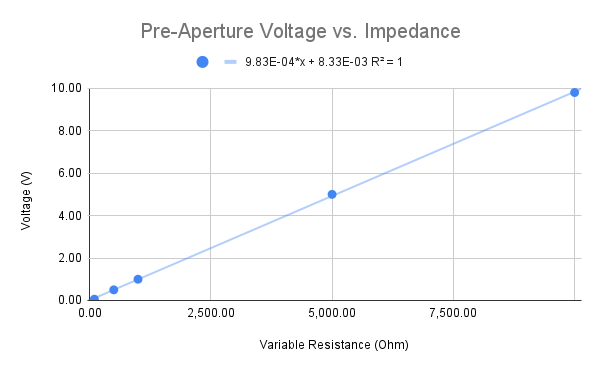
\includegraphics[width=0.75\linewidth]{Resources//180Q//Homework 2/Pre-Aperture Voltage vs. Impedance.png}
    \caption{Voltage (V) vs. Resistance (Ohms) of photodiode on laser input.}
    \label{fig:enter-label}
\end{figure}

\pagebreak
\subsection*{Part c}
The power after the first aperture is $563nW$ and the power after the second aperture is $40.3nW$.
\begin{figure}[h]
    \centering
    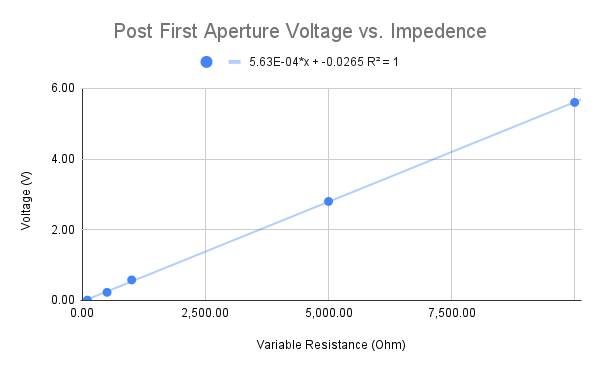
\includegraphics[width=0.75\linewidth]{Resources//180Q//Homework 2/Post First Aperture Voltage vs. Impedence.png}
    \caption{Voltage vs. resistance after first aperture.}
    \label{fig:enter-label}
\end{figure}
\begin{figure}[h]
    \centering
    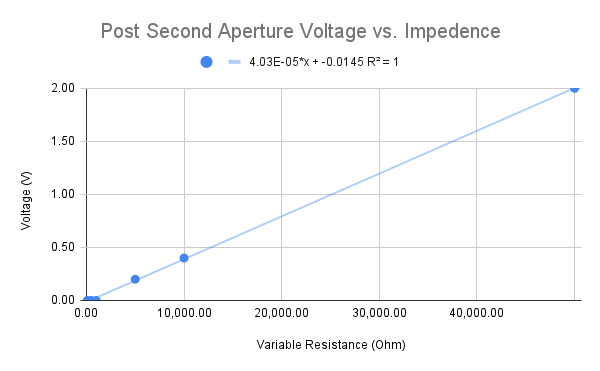
\includegraphics[width=0.75\linewidth]{Resources//180Q//Homework 2/Post Second Aperture Voltage vs. Impedence.png}
    \caption{Voltage vs. resistance after second aperture.}
    \label{fig:enter-label}
\end{figure}

The fraction of light that makes it through the first aperture is
$$
\eta_1 = \frac{563nW}{983nW} \approx 0.573
$$

The fraction of light that makes it through the second aperture is
$$
\eta_2 = \frac{40.3nW}{563nW} \approx 0.0716
$$

\pagebreak
\usection{Aligning a lens to a beam}

\subsection*{Part a}
After adding the focusing lens the power after the second aperture is $585nW$.
\begin{figure}[h]
    \centering
    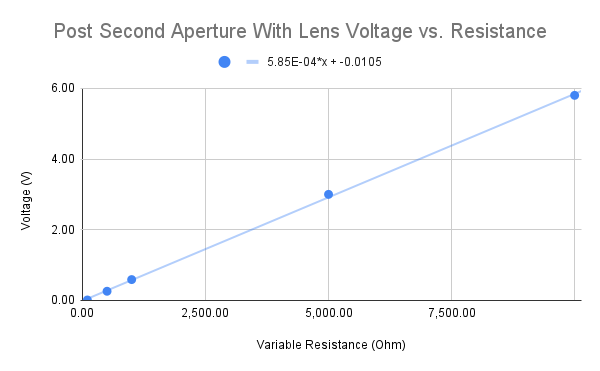
\includegraphics[width=0.75\linewidth]{Resources//180Q//Homework 2/Post Second Aperture With Lens Voltage vs. Resistance.png}
    \caption{Voltage vs. resistance after second aperture.}
    \label{fig:enter-label}
\end{figure}

The new coupling efficiency now $\eta_2 \approx 1$\footnote{Relative to our previous power measurement, it would suggest that $\eta_2 > 1$! However, this is just from both the laser source and the first aperture being bumped at some point.}. Previously, most of the light was blocked by the aperture, after adding the lens nearly all of the light is passed through the aperture hole.

\pagebreak
\subsection*{Part c}
The back reflected power is $5.68nW$. The incident power is $563nW$.
\begin{figure}[h]
    \centering
    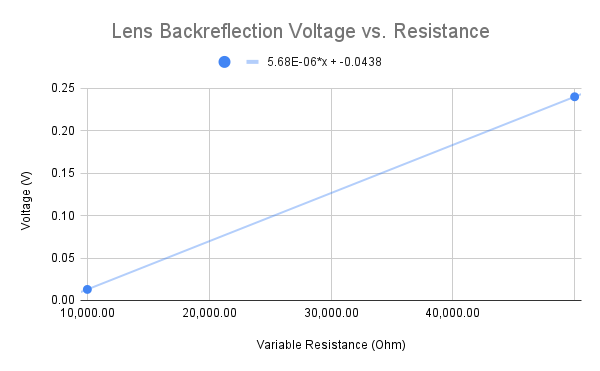
\includegraphics[width=0.75\linewidth]{Resources//180Q//Homework 2/Lens Backreflection Voltage vs. Resistance.png}
    \caption{Back reflection power from lens.}
    \label{fig:enter-label}
\end{figure}
The fraction of power reflection is
$$
\eta_{ref} = \frac{5.68nW}{563nW} \approx 0.0100
$$

\subsection*{Part d}
In the pre-lab we estimated that we would loose about $7\%$ of the incident power, $10\%$, makes sense if we also consider surface diffusion.

\pagebreak
\usection{Aligning a beam splitter}

\subsection*{Part a}
The output power is $20.1nW$ and the input power is $40.3nW$, so we're measuring a transmission of
$$
\eta_{bs} = \frac{20.1}{40.3} \approx 0.499
$$

\begin{figure}[h]
    \centering
    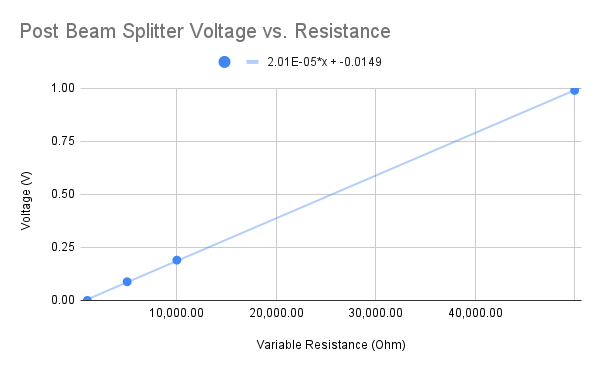
\includegraphics[width=0.75\linewidth]{Resources//180Q//Homework 2/Post Beam Splitter Voltage vs. Resistance.png}
    \caption{Post beam splitter voltage vs. resistance.}
    \label{fig:enter-label}
\end{figure}
